\section{Ultrafast PSYCHE-iDOSY}
\label{sec:pureshift__epsidosy}

In the final section of this chapter, I turn to something entirely different: the combination of pure shift diffusion NMR with ultrafast acquisition.
This work was done in collaboration with \JND{} (University of Nantes): the original project idea was first conceived and implemented there.
Unfortunately, the results we obtained at Oxford were not promising enough to drive the project further, especially in light of time constraints.
However, for the sake of completeness, I describe the overall concept as well as these results in this section.

\begin{figure}[htb]
    \centering
    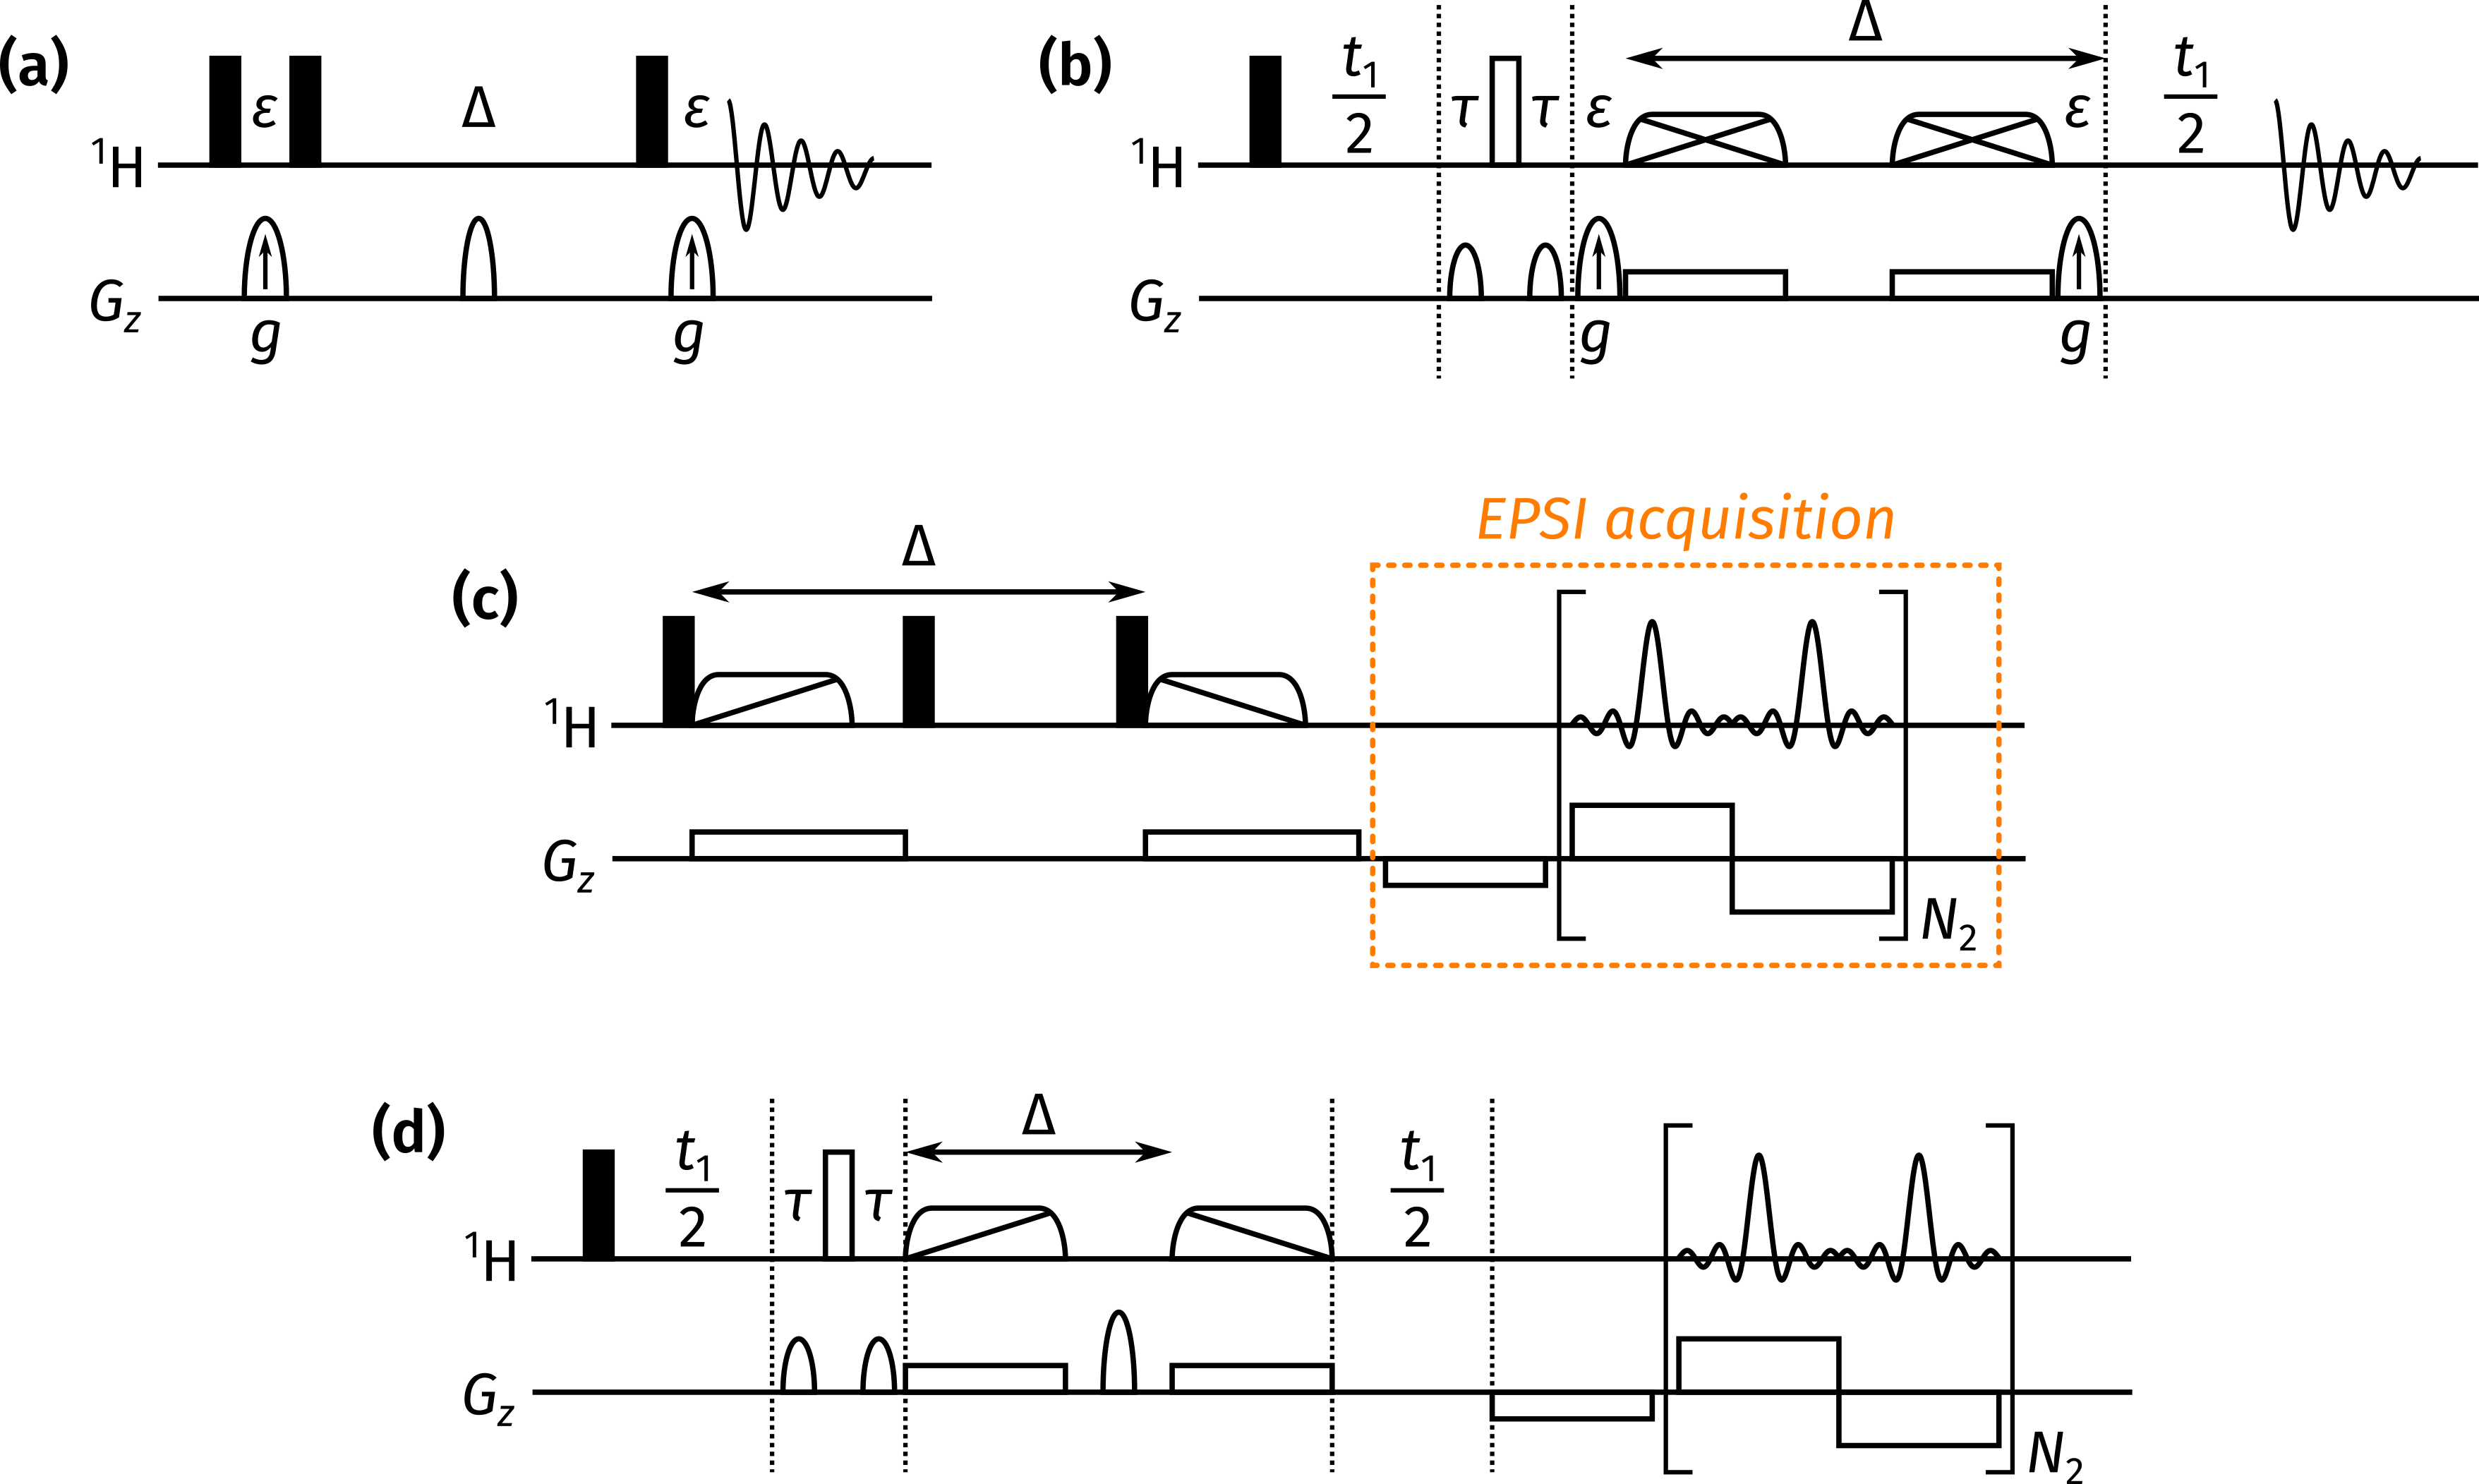
\includegraphics[]{pp/pureshift/epd_pulseq.png}%
    {\phantomsubcaption\label{fig:epd_pulseq_stedosy}}%
    {\phantomsubcaption\label{fig:epd_pulseq_psychedosy}}%
    {\phantomsubcaption\label{fig:epd_pulseq_epsidosy}}%
    {\phantomsubcaption\label{fig:epd_pulseq_epsipsychedosy}}%
    \caption[EPSI PSYCHE-iDOSY and associated pulse sequences]{
        \textbf{(\subref{fig:epd_pulseq_stedosy})} Basic stimulated echo DOSY experiment.
        To acquire the diffusion dimension, the amplitudes of gradients with arrows inside are incremented.
        $\Delta$ indicates the diffusion delay.
        \textbf{(\subref{fig:epd_pulseq_psychedosy})} PSYCHE-iDOSY experiment. $\tau$ is set to $1/(4 \cdot T_\text{chunk})$, as before.
        \textbf{(\subref{fig:epd_pulseq_epsidosy})} Ultrafast DOSY experiment. The EPSI acquisition block is highlighted in orange, consisting of a prephasing gradient followed by detection in the presence of alternating gradients.
        \textbf{(\subref{fig:epd_pulseq_epsipsychedosy})} Ultrafast PSYCHE-iDOSY experiment. Note the use of unidirectional chirps rather than saltire pulses.
    }
    \label{fig:epd_pulseq}
\end{figure}

I begin with a brief overview of diffusion NMR\autocite{Johnson1999PNMRS}; this topic will also be covered in some detail in \cref{subsec:poise__diffusion}.
\Cref{fig:epd_pulseq_stedosy} shows a typical 2D stimulated echo DOSY experiment, where the indirect (diffusion) dimension involves the incrementation of gradient amplitudes rather than an evolution delay.
For each gradient amplitude, one time-domain signal is recorded.
Molecular diffusion during a delay placed between a pair of gradients leads to attenuation of the signal, as the spatially-dependent phase imparted by the first gradient is not perfectly refocused by the second.
This attenuation is described by the Stejskal--Tanner equation\autocite{Stejskal1965JCP,Sinnaeve2012CMR}, which in its simplest form is:
\begin{equation}
    \label{eq:stejskal_tanner}
    I(G) = I(0) \exp\left[-(\gamma\delta G)^2 D \Delta'\right].
\end{equation}
Here, $I(G)$ represents the signal intensity when measured with a gradient amplitude of $G\/$; $\gamma$ is the magnetogyric ratio, $\delta$ is the duration of the bracketing gradients, $D\/$ the diffusion coefficient, and $\Delta'$ a `corrected' diffusion delay.
The exact correction required depends on the shapes of the gradients used.
By measuring the signal intensity $I\/$ for at least two different values of $G\/$, the diffusion coefficient $D\/$ can be estimated.%
\footnote{As will be discussed in \cref{subsec:poise__diffusion}, this should really be an \textit{apparent} diffusion coefficient as there are various other factors which can affect the intensity, notably convection.}

The fact that different molecules have different diffusion coefficients, and thus different attenuation profiles, can be used to separate mixtures of molecules through the basic DOSY experiment.
However, when signals from different species overlap in the \proton{} spectrum, (as is often the case in mixtures), it is not possible to cleanly extract the separate peak intensities, resulting in poor resolution in the diffusion dimension.
There are several ways to solve this issue: for example, peaks can be resolved using another chemical shift dimension in a 3D experiment.\autociteset{3ddosy}
A slightly less time-consuming option is pure shift NMR.
The first pure shift diffusion experiments used either the \ang{45} projection of a 2DJ spectrum\autocite{Cobas2004JMR}, or the Zangger--Sterk PSE\autocite{Nilsson2007CC,Aguilar2010ACIE,Glanzer2014CEJ}: in both cases, improvements in the resolution of diffusion coefficients were reported.
The PSYCHE-iDOSY experiment\autocite{Foroozandeh2016ACIE} (\cref{fig:epd_pulseq_psychedosy}) improved upon these, much in the same way that PSYCHE itself improved on existing pure shift methods.
The `i' refers to the fact that the diffusion delay is \textit{internal} to the sequence, i.e.\ it is simply added in the middle of the PSYCHE element, which (using the instantaneous flip approximation) can itself be thought of as a spatially parallel stimulated echo.
This avoids the need to add an entirely separate stimulated echo at the beginning or end of the sequence.

While the addition of a pure shift dimension is less expensive compared to a full chemical shift dimension in terms of time, the fact remains that the PSYCHE-iDOSY is a (pseudo)-3D experiment.
One way to shorten this is to use spatial encoding techniques to collapse one dimension, specifically the diffusion dimension\autocite{Telkki2021PNMRS}.
Two separate steps are required for this: firstly, a gradient whose amplitude varies across the sample must be applied (the `encoding' step), and then an imaging acquisition technique must be used to read out the signal in each slice of the sample (the `detection' step).
This was first done by Loening et al.\autocite{Loening2001JMR}, where the encoding was performed using the field generated by a $z^2$ shim coil.
The readout was then performed by simply acquiring the FID in the presence of a weak gradient, such that the peak shapes directly reflect the distribution of signal intensities across the sample.
Later, Thrippleton et al.\autocite{Thrippleton2003MRC} introduced the (by now familiar) chirp--gradient combination for spatial encoding: since spins in different slices are inverted at different times, the total gradient area applied in each slice is different.
In later work by the groups of Frydman\autocite{Shrot2008JMR} and Dumez\autocite{Guduff2017CC,Jacquemmoz2022MRC}, the spatial encoding of the diffusion attenuation is still accomplished using the very same chirp--gradient combination.
However, the detection is accomplished using the \ac{epsi} acquisition technique\autocite{Mansfield1977JPCSSP,Stehling1991S}, much like in ultrafast 2D NMR (\cref{fig:epd_pulseq_epsidosy})\autociteset{ultrafast}.

Unsurprisingly, the aim in this section is to unite the PSYCHE-iDOSY and ultrafast DOSY techniques to form an ultrafast PSYCHE-iDOSY experiment.
This would yield PSYCHE-iDOSY spectra in a much reduced time, at the cost of sensitivity.
The resulting pulse sequence is shown in \cref{fig:epd_pulseq_epsipsychedosy}.
The EPSI acquisition is used to collapse the diffusion dimension, not the PSYCHE chunking dimension.%
\footnote{The other option would require an ultrafast PSYCHE experiment, which---to date---has not been developed.}
One benefit of this is that only one PSYCHE chunk needs to be acquired at a time, circumventing the need for long EPSI detection periods (which can cause spectrometer damage).
Note also that it is mandatory to use unidirectional chirps in the PSYCHE PSE: in the original PSYCHE-iDOSY, these pulses were used only for homonuclear decoupling, and thus saltire pulses were acceptable (indeed, superior).
However, in the ultrafast version, the PSE is also responsible for creating the requisite spatial encoding of gradient areas.
Using saltire pulses here would lead to an undesired `double' encoding, yielding data which cannot be processed correctly.

The sequence itself was written and evaluated by Corentin Jacquemmoz and \JND{} at the University of Nantes, on a concentrated (\qty{1}{\molar}) sample of ethanol in \ch{D2O}.
Their results are shown in \cref{fig:epsi_jnd_mf_jnd_kt,fig:epsi_jnd_mf_jnd_zd,fig:epsi_jnd_mf_jnd_trace}.
When I later tried to reproduce these results, I additionally used the POISE routine described in \cref{subsec:poise__epsi} to optimise the amplitude ratio between the positive and negative gradients during the EPSI acquisition (without optimisation, the results obtained were even poorer); my results are shown in \cref{fig:epsi_jnd_mf_mf_kt,fig:epsi_jnd_mf_mf_zd,fig:epsi_jnd_mf_mf_trace}.
The data processing used to generate these figures was written by me,\footnote{The Nantes team have a more complete Matlab package for this, which goes several steps further than that shown here and includes features such as phase correction and fitting of the diffusion profiles to various (though not yet fully appropriate) Stejskal--Tanner equations. However, these were not necessary here as the project never got to that stage, and I preferred to use Python.} and broadly consists of the following steps: reshaping of the EPSI raw data, concatenation of PSYCHE chunks, and Fourier transformation in both dimensions.%
\footnote{As discussed in Frydman et al.\autocite{Frydman2003JACS}, the $k$-domain in ultrafast NMR is directly proportional to the indirect-dimension frequency domain. So, to obtain the diffusion profile---which varies with space, i.e. $z$---a Fourier transform along this axis is required.}
For simplicity, the data points acquired during the negative gradients is discarded.

\begin{figure}[htbp]
    \centering
    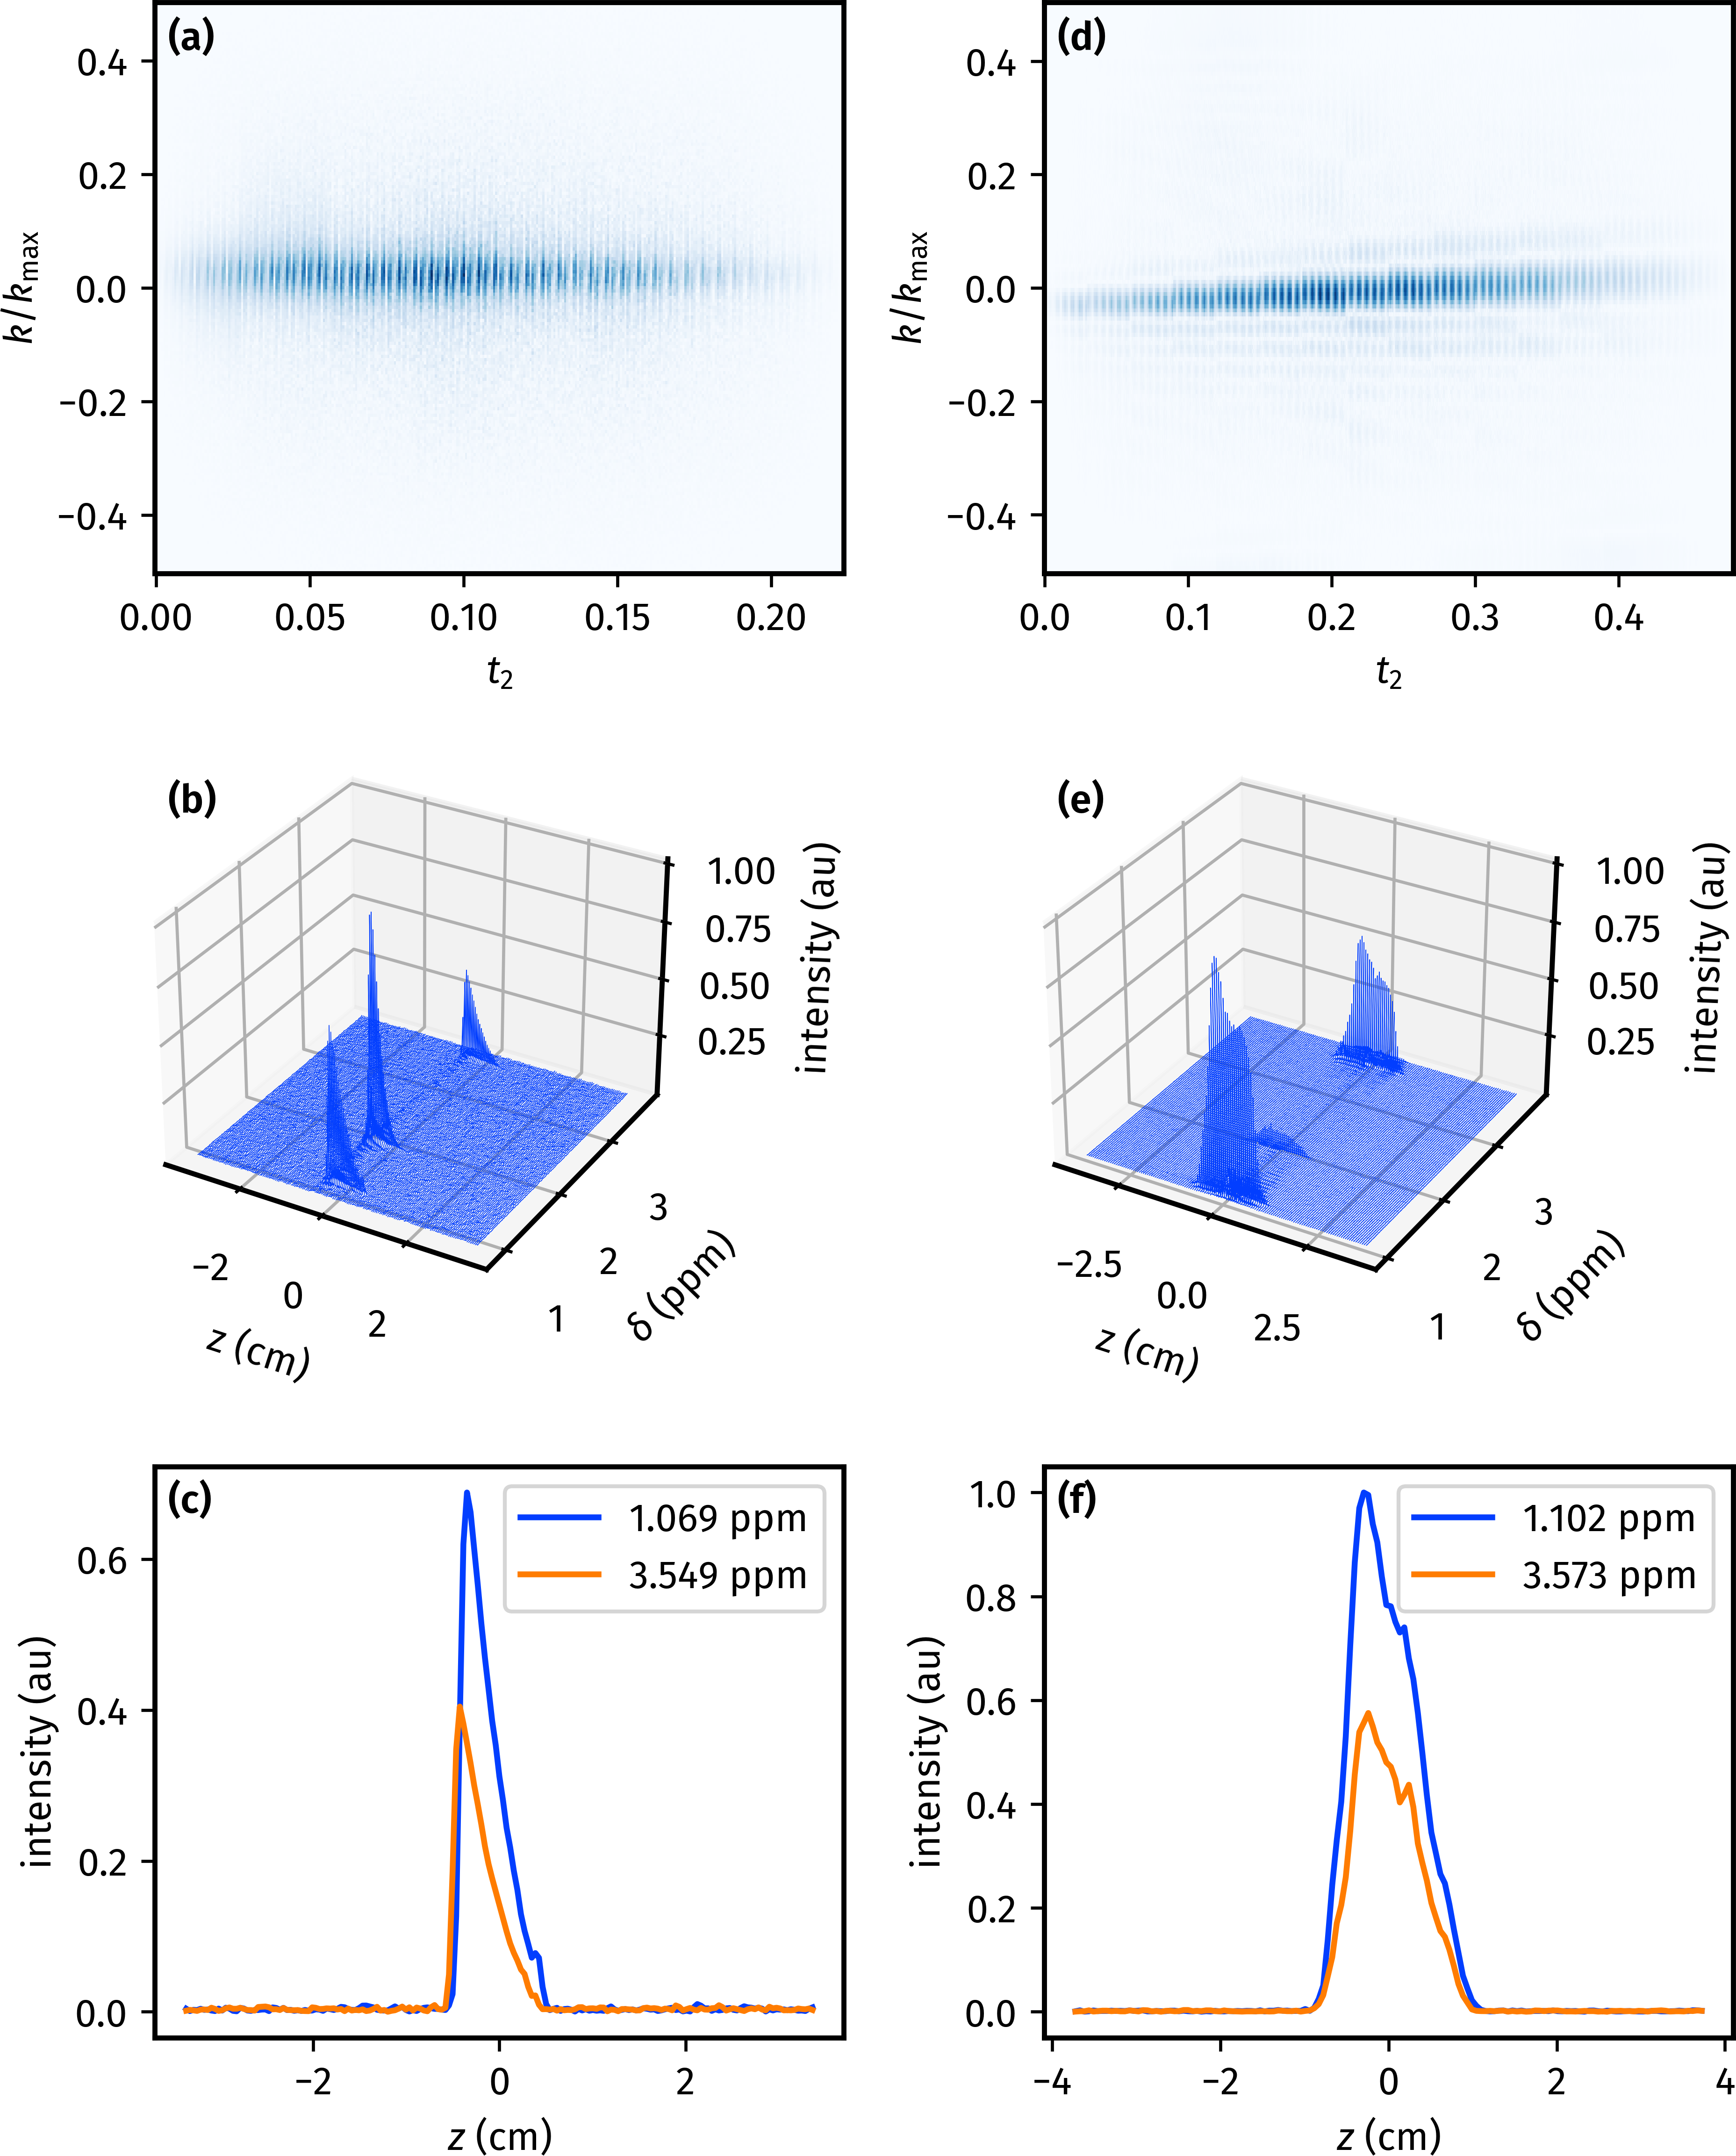
\includegraphics[]{pureshift/epsi_jnd_mf.png}%
    {\phantomsubcaption\label{fig:epsi_jnd_mf_jnd_kt}}%
    {\phantomsubcaption\label{fig:epsi_jnd_mf_jnd_zd}}%
    {\phantomsubcaption\label{fig:epsi_jnd_mf_jnd_trace}}%
    {\phantomsubcaption\label{fig:epsi_jnd_mf_mf_kt}}%
    {\phantomsubcaption\label{fig:epsi_jnd_mf_mf_zd}}%
    {\phantomsubcaption\label{fig:epsi_jnd_mf_mf_trace}}%
    \caption[Comparison of EPSI PSYCHE-iDOSY data acquired in Nantes and Oxford]{
        \textbf{(\subref{fig:epsi_jnd_mf_jnd_kt})--(\subref{fig:epsi_jnd_mf_jnd_trace})} EPSI PSYCHE-iDOSY data obtained by Corentin Jacquemmoz and \JND{} at the University of Nantes.
        The three plots respectively show the 2D raw $(k, t_2)$ data (after PSYCHE processing has been carried out); the Fourier transformed $(z, \delta)$ data; and the individual diffusion profiles for each peak.
        \textbf{(\subref{fig:epsi_jnd_mf_mf_kt})--(\subref{fig:epsi_jnd_mf_mf_trace})} The equivalent data which I recorded in Oxford.
        The central peak corresponds to \ch{HDO}; the Oxford sample used was drier and thus it is less intense in (\subref{fig:epsi_jnd_mf_mf_zd}) compared to (\subref{fig:epsi_jnd_mf_jnd_zd}).
        \datacode{6E-210426}
    }
    \label{fig:epsi_jnd_mf}
\end{figure}

In principle, the Fourier transformed $(z, \delta)$ plots should reveal a diffusion profile similar to that in Guduff et al.\autocite{Guduff2017CC}
This is the case for the Nantes data; in fact, it was possible to process this further to obtain a conventional 2D DOSY spectrum, where the diffusion coefficient for each component is extracted and plotted.
For the Oxford data, although the general \textit{form} of the curve is correct (in that there is a generally decreasing pattern), there are clearly `spikes' in the $(z,\delta)$ diffusion profiles.

My current best hypothesis is that these spikes are artefacts from unwanted CTPs which are ordinarily suppressed through spatial averaging, but are instead being refocused by the gradients during the EPSI acquisition.
This is supported by the fact that the Nantes data was acquired on a microimaging probe equipped with triaxial gradients, which allowed CTP gradients to be applied along the $x$- and $y$-axes (note that the PSYCHE gradient must still be applied along the $z$-axis).
Naturally, any artefacts dephased by these cannot be refocused by the $z$-gradients in the EPSI block.
On the other hand, the Oxford data was acquired on a Prodigy cryoprobe with only $z$-gradients.

The intensity of these `spike' artefacts can, in fact, be controlled by varying other acquisition parameters.
For example, increasing the EPSI gradient amplitude leads to increased artefacts (\cref{fig:epsi_parameters_moreepsi_kt,fig:epsi_parameters_moreepsi_trace}): this lends credence to the hypothesis above that the artefacts arise from refocused CTPs.
Notice also the appearance of signals at $k \neq 0$: this should not happen because in ultrafast experiments, the $k$-axis is proportional to the evolution frequency as a function of $z$ (i.e. indirect-dimension frequencies in a typical 2D experiment).
In a diffusion experiment, however, there is no frequency modulation in the indirect or spatial dimension, only amplitude modulation arising from diffusion attenuation; so, all signals should fall along $k = 0$.
In principle, the EPSI gradient could instead be reduced, but this has the drawback of lowering the resolution in the diffusion dimension.
Alternatively, when the PSYCHE gradient is increased, the artefacts seem to be reduced (\cref{fig:epsi_parameters_morepsyche_kt,fig:epsi_parameters_morepsyche_trace}).
However, this cannot be varied too much as the PSYCHE gradients are also responsible for the diffusion encoding (the value of $g$ in the Stejskal--Tanner equation are effectively derived from this).

\begin{figure}[htb]
    \centering
    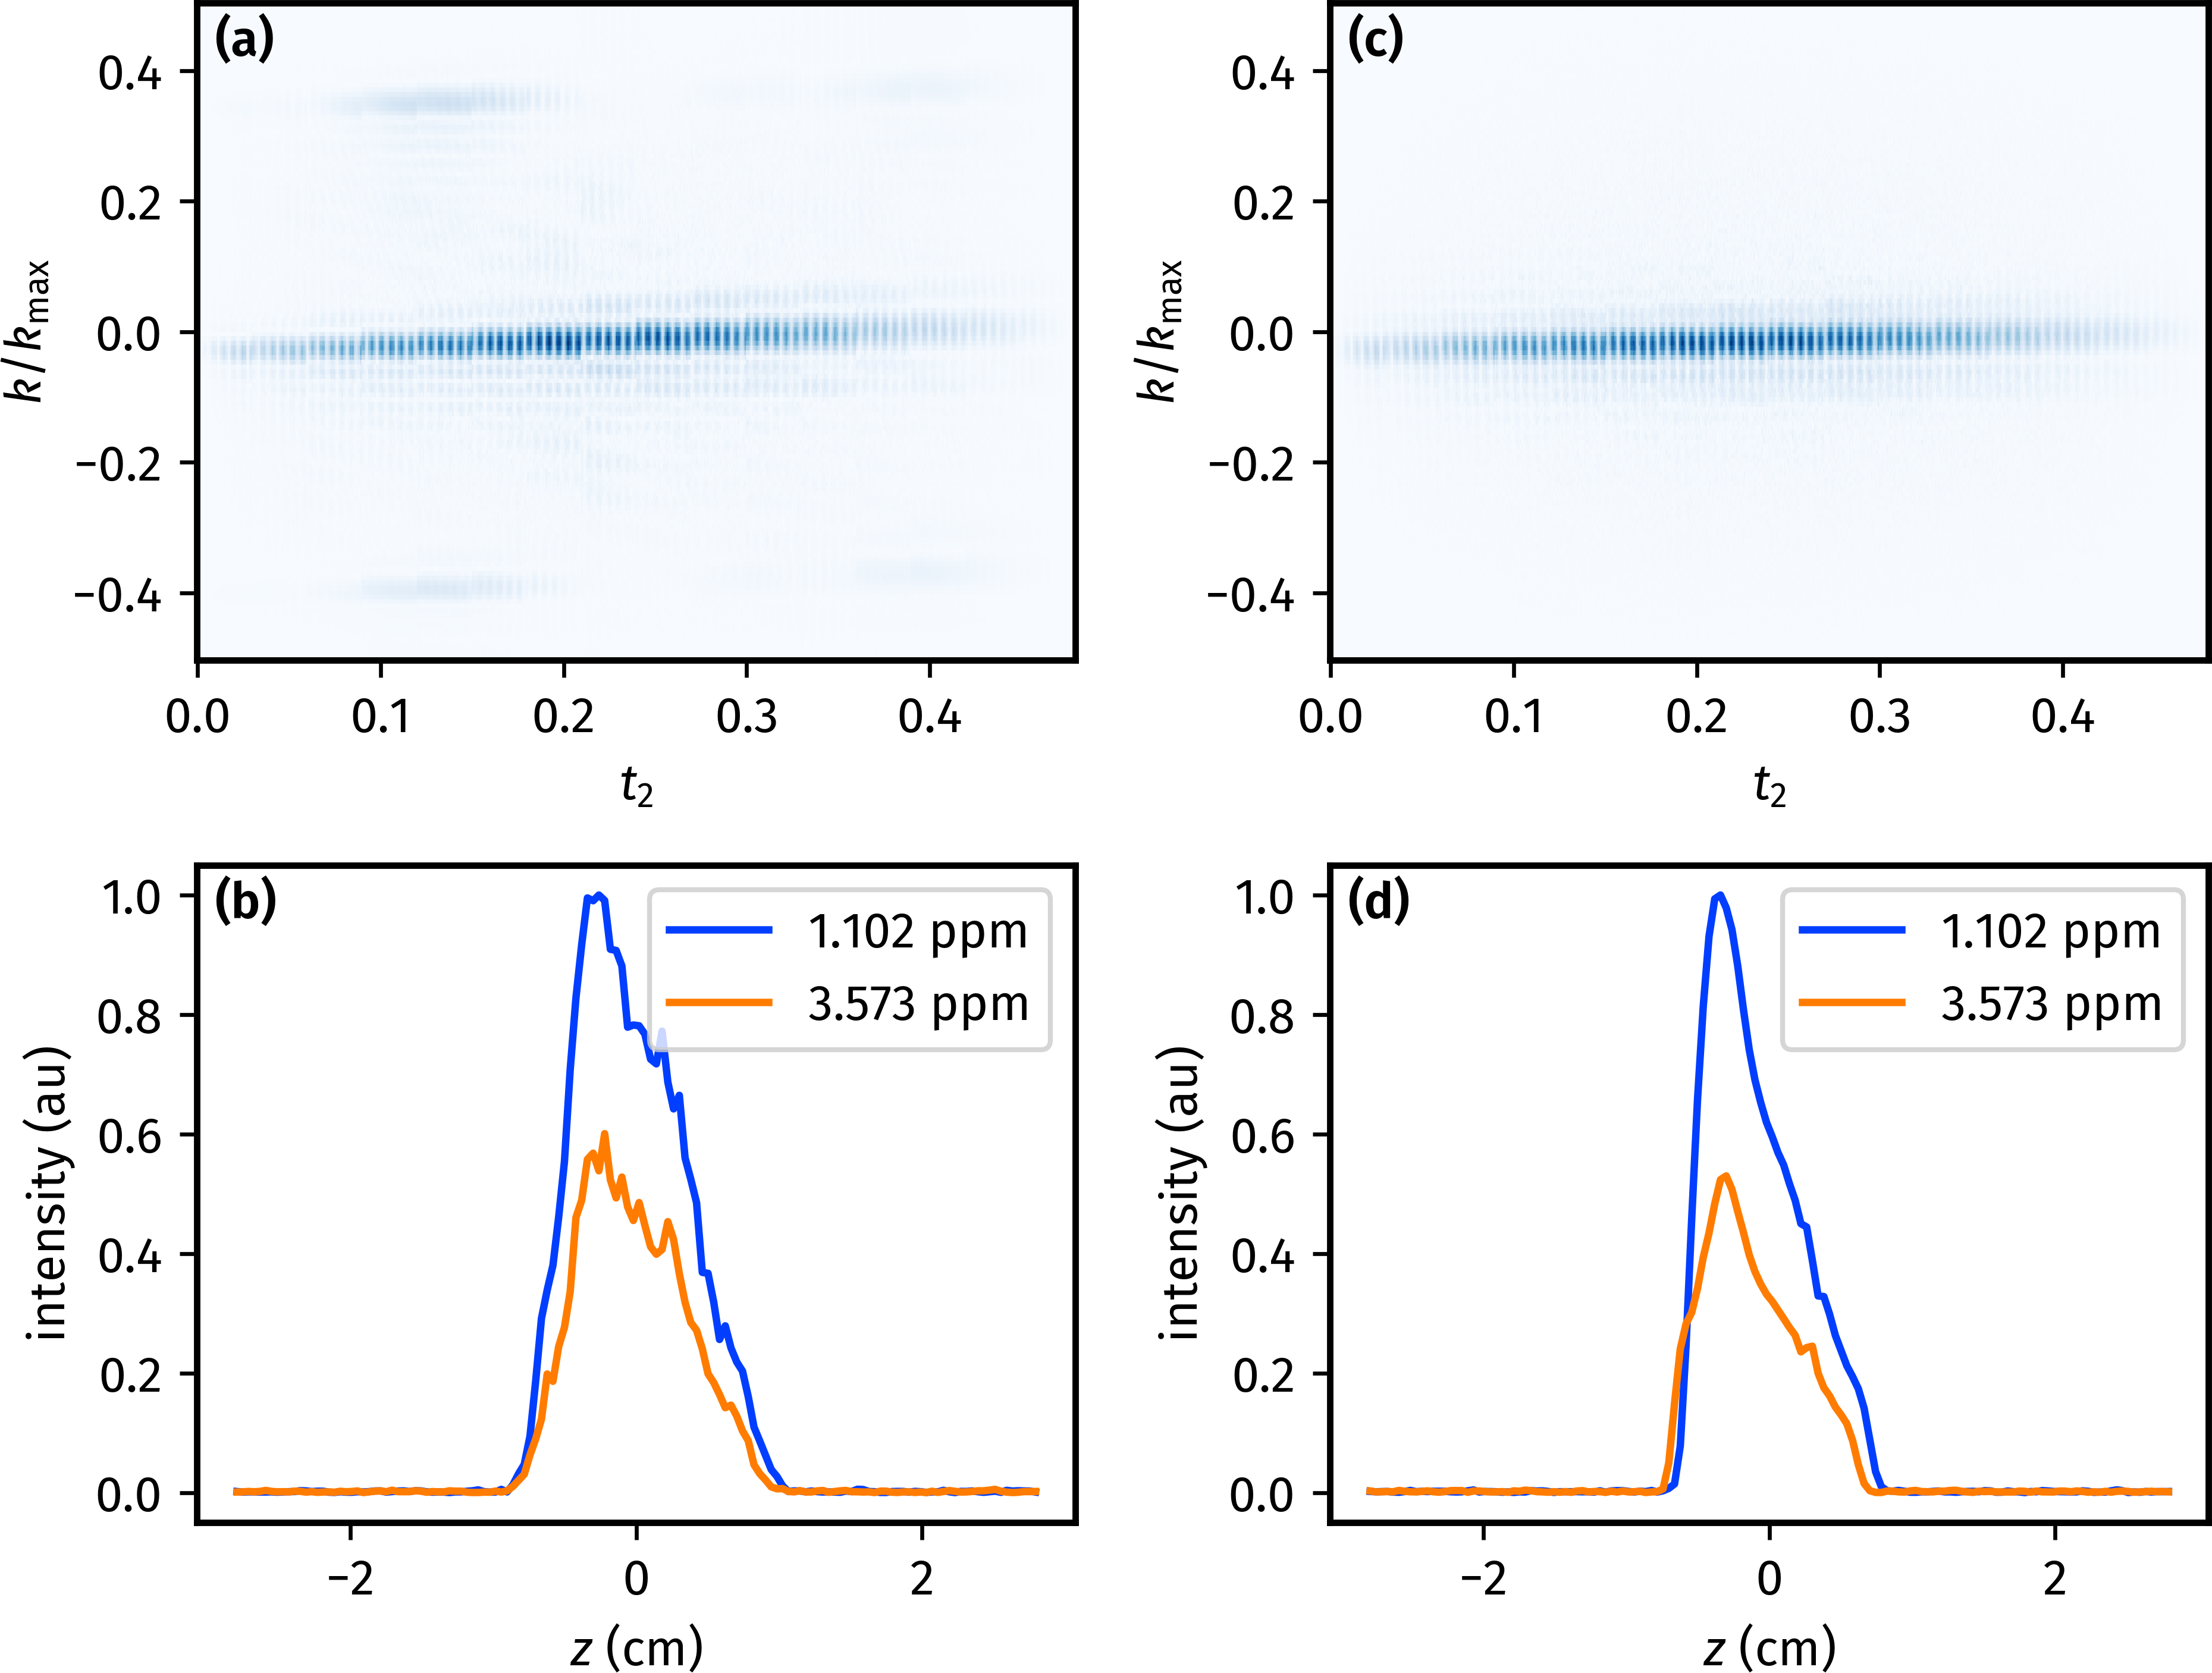
\includegraphics[]{pureshift/epsi_parameters.png}%
    {\phantomsubcaption\label{fig:epsi_parameters_moreepsi_kt}}%
    {\phantomsubcaption\label{fig:epsi_parameters_moreepsi_trace}}%
    {\phantomsubcaption\label{fig:epsi_parameters_morepsyche_kt}}%
    {\phantomsubcaption\label{fig:epsi_parameters_morepsyche_trace}}%
    \caption[Effects of varying acquisition parameters on ultrafast PSYCHE-iDOSY spectra]{
        \textbf{(\subref{fig:epsi_parameters_moreepsi_kt})--(\subref{fig:epsi_parameters_moreepsi_trace})} The same as in \cref{fig:epsi_jnd_mf_mf_kt,fig:epsi_jnd_mf_mf_trace}, but with the EPSI acquisition gradient increased to 32\% (from 24\% in the original).
        \datacode{6E-210426}
        \textbf{(\subref{fig:epsi_parameters_morepsyche_kt})--(\subref{fig:epsi_parameters_morepsyche_trace})} The same as in \cref{fig:epsi_jnd_mf_mf_kt,fig:epsi_jnd_mf_mf_trace}, but with the PSYCHE gradient increased to 5\% (from 3\% in the original).        
        \datacode{6E-210505}
    }
    \label{fig:epsi_parameters}
\end{figure}

Another possible reason for the artefacts is a potentially poorer $B_1$ homogeneity on the Oxford instrument.
However, a simple pulse--EPSI experiment (\cref{fig:zg_epsi}) shows that the $B_1$ spatial profile, though not perfect, is relatively uniform.

\begin{figure}[htb]
    \centering
    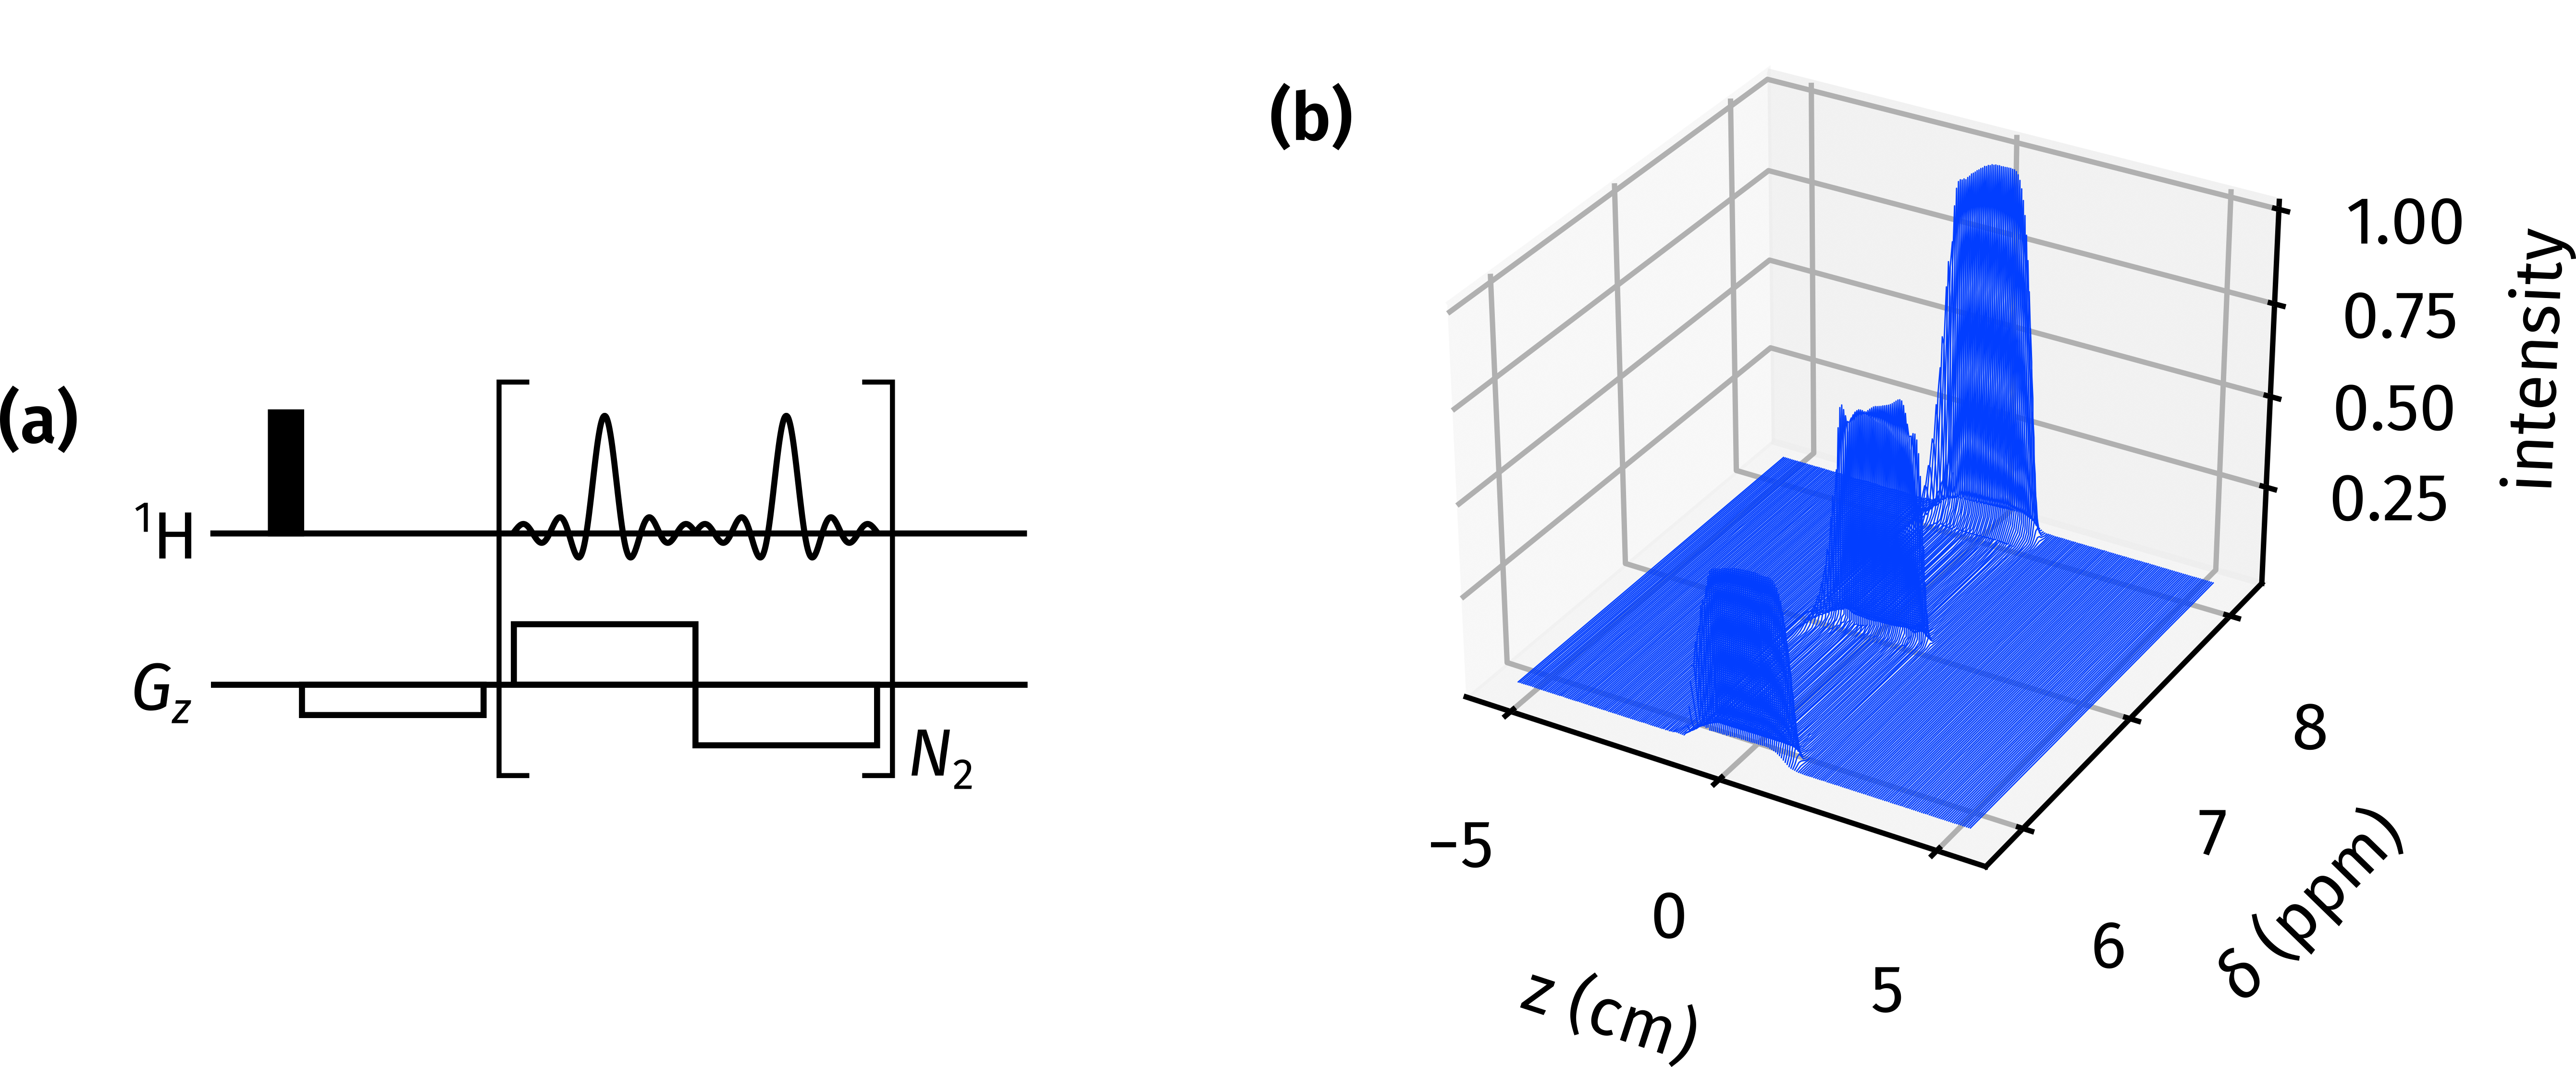
\includegraphics[]{pureshift/zg_epsi.png}%
    {\phantomsubcaption\label{fig:zg_epsi_pulseq}}%
    {\phantomsubcaption\label{fig:zg_epsi_spec}}%
    \caption[Pulse--EPSI pulse sequence and data]{
        \textbf{(\subref{fig:zg_epsi_pulseq})} Pulse--EPSI pulse sequence. The variation of the peak intensity along the $z$-axis directly corresponds to the $B_1$ spatial profile.
        \textbf{(\subref{fig:zg_epsi_spec})} The resulting data after Fourier transformation in both dimensions ($k \leftrightarrow z$ and $t_2 \leftrightarrow \delta$).
        \datacode{6E-210426}
    }
    \label{fig:zg_epsi}
\end{figure}

Curiously, \cref{fig:epsi_jnd_mf_mf_kt} shows that in the Oxford data, there is a progressive `shifting' along the $k$-axis in each PSYCHE chunk.
(The POISE optimisation in \cref{subsec:poise__epsi} was used to correct for the drifting \textit{within} each chunk, but cannot be applied to the overall drift after the concatenation of chunks.)
One possible explanation for this is perhaps lingering effects from gradients applied during the pulse sequence, which have more time to dissipate when $t_1$ is longer.
This, however, does not have an appreciable impact on the data: it can be crudely corrected by circularly shifting the data along the $k$-axis by an appropriate amount, and Fourier transformation of the resulting data yielded effectively the same results.

All in all, it appears that the fundamental idea behind the ultrafast PSYCHE-iDOSY experiment is sound: the Nantes data is an excellent proof-of-principle.
However, the implementation of the sequence almost certainly needs to be optimised in order for high-quality data to be extracted.
An important subsequent step would then be to derive the appropriate form of the Stejskal--Tanner equation for extracting diffusion coefficients from the data.
Sadly, I simply did not quite have the time to pursue this in further detail.
